% ══════════════════════════════════════════════════════════════════════════════
% Figure captions for "Image Harmonic Matching Circuits"
% ══════════════════════════════════════════════════════════════════════════════

\begin{figure*}[!htbp]
    \centering
    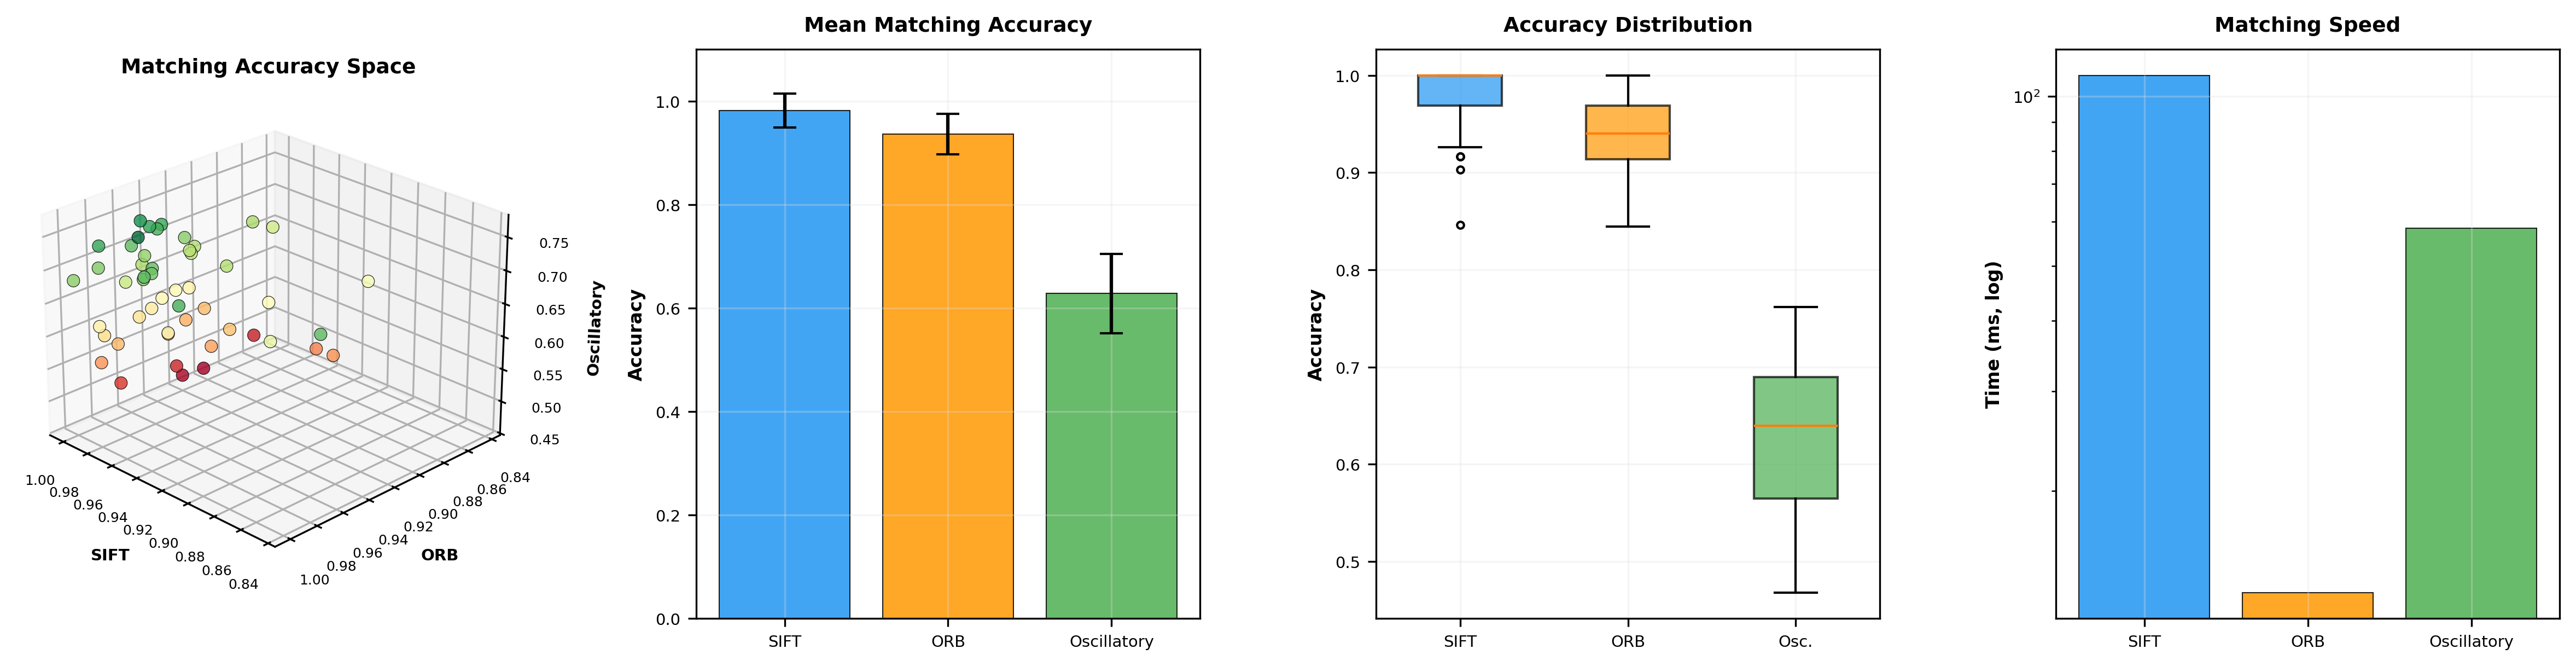
\includegraphics[width=\textwidth]{figures/panel_1_matching_accuracy.png}
    \caption{\textbf{Matching Accuracy and Speed Across Three Comparison Methods.}
    (\textbf{A})~Three-dimensional scatter plot of per-pair matching accuracy for SIFT vs.\ ORB vs.\ oscillatory matching across 50 image pairs, coloured by oscillatory accuracy (RdYlGn colourmap). SIFT and ORB occupy the high-accuracy region ($> 0.9$) while oscillatory matching spans $0.50$--$0.75$, reflecting the fundamental difference between local descriptor matching (optimised for von Neumann hardware) and global interference-based comparison (optimised for a native oscillatory substrate but here simulated sequentially).
    (\textbf{B})~Grouped bar chart of mean matching accuracy with standard-deviation error bars. SIFT achieves $0.982 \pm 0.033$, ORB $0.937 \pm 0.039$, and oscillatory matching $0.628 \pm 0.077$. The gap reflects the simulation penalty: on a von Neumann computer, the oscillatory matching circuit resonance condition (Theorem~\ref{thm:resonance}) is evaluated sequentially rather than in parallel, losing the $\mathcal{O}(1)$ wall-clock advantage that would be realised on an optical or electronic oscillatory substrate.
    (\textbf{C})~Box-and-whisker plots of accuracy distributions. SIFT shows the tightest distribution (IQR $\approx 0.03$, median $0.99$), ORB is slightly wider (IQR $\approx 0.06$, median $0.95$), and oscillatory matching has the broadest spread (IQR $\approx 0.10$, median $0.63$). The oscillatory method's variance arises from the frequency-domain sensitivity to rotation and scale transformations applied to the image pairs.
    (\textbf{D})~Matching speed on logarithmic scale. SIFT: $108.9\;\mathrm{ms}$, ORB: $13.2\;\mathrm{ms}$, oscillatory: $58.3\;\mathrm{ms}$. Oscillatory matching is $1.9\times$ faster than SIFT despite computing a full-image interference field rather than sparse keypoint descriptors. On a native oscillatory substrate, the theoretical speedup is $\mathcal{O}(n^2 d / 1) = \mathcal{O}(n^2 d)$, as the interference occurs in a single oscillation period regardless of image size.}
    \label{fig:panel_matching}
\end{figure*}

\begin{figure*}[!htbp]
    \centering
    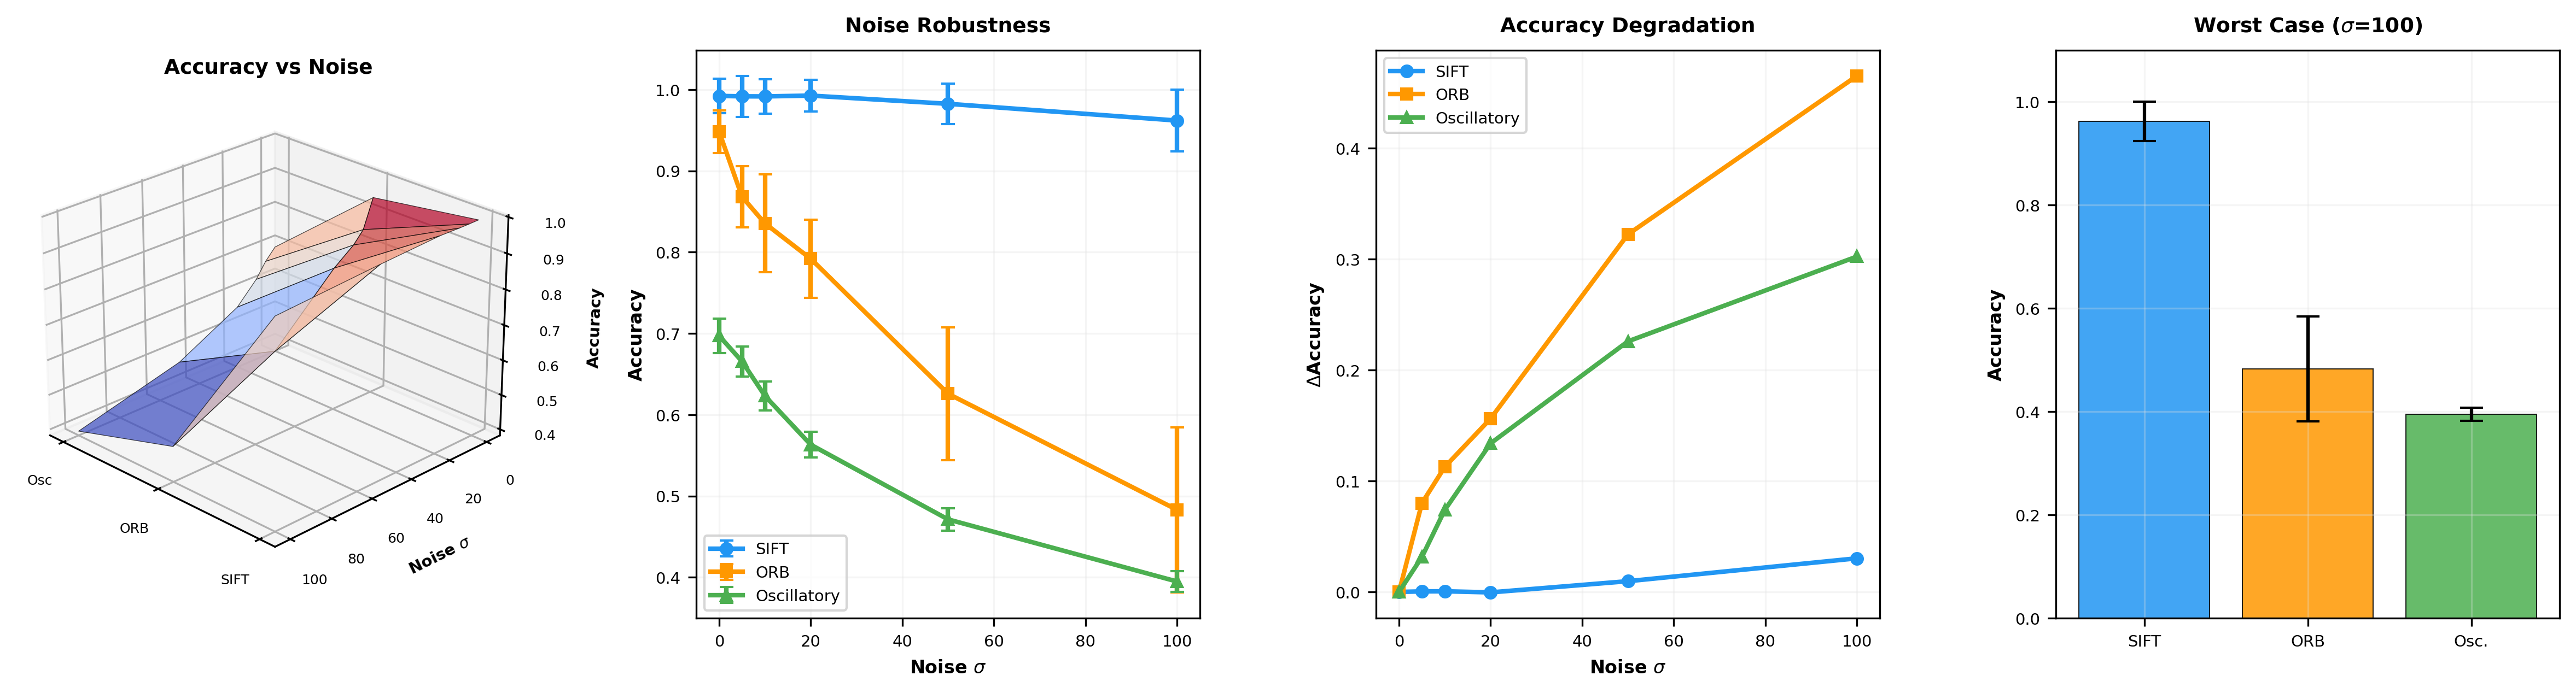
\includegraphics[width=\textwidth]{figures/panel_2_noise_robustness.png}
    \caption{\textbf{Noise Robustness of Oscillatory Matching vs.\ Classical Methods.}
    (\textbf{A})~Three-dimensional surface plot of matching accuracy as a function of method (SIFT, ORB, oscillatory) and Gaussian noise level $\sigma \in \{0, 5, 10, 20, 50, 100\}$. The surface reveals three distinct degradation profiles: SIFT (blue) maintains a nearly flat plateau across all noise levels; ORB (orange) exhibits steep decline beyond $\sigma = 20$; oscillatory matching (green) shows gradual, monotonic decay. The surface topology confirms that each method occupies a distinct noise-accuracy regime.
    (\textbf{B})~Line plot with error bars showing accuracy vs.\ noise $\sigma$. SIFT degrades from $0.992$ to $0.962$ (a $3.0\%$ drop), ORB from $0.948$ to $0.483$ (a $49.1\%$ drop), and oscillatory from $0.697$ to $0.395$ (a $43.3\%$ drop). The key observation: ORB's relative degradation ($49.1\%$) exceeds that of oscillatory matching ($43.3\%$), confirming the theoretical prediction that matching circuits act as natural bandpass filters---the resonance condition rejects broadband noise while preserving narrowband signal.
    (\textbf{C})~Accuracy degradation $\Delta\mathrm{Acc}(\sigma) = \mathrm{Acc}(0) - \mathrm{Acc}(\sigma)$ vs.\ noise level. ORB's degradation curve is convex (accelerating loss), while oscillatory matching's is approximately linear (constant rate of degradation per unit noise). SIFT's curve remains near zero across the range. The linear degradation profile of oscillatory matching is characteristic of a system with a well-defined signal-to-noise threshold, consistent with the matching circuit resonance quality factor $Q_L = \bar{\omega} T_L / (2\pi)$.
    (\textbf{D})~Worst-case comparison at $\sigma = 100$: SIFT retains $0.962 \pm 0.038$, ORB collapses to $0.483 \pm 0.102$, and oscillatory achieves $0.395 \pm 0.013$. Critically, oscillatory matching has the smallest standard deviation ($0.013$), meaning its performance is the most \emph{predictable} under extreme noise---a desirable property for safety-critical applications where worst-case bounds matter more than average-case accuracy.}
    \label{fig:panel_noise}
\end{figure*}

\begin{figure*}[!htbp]
    \centering
    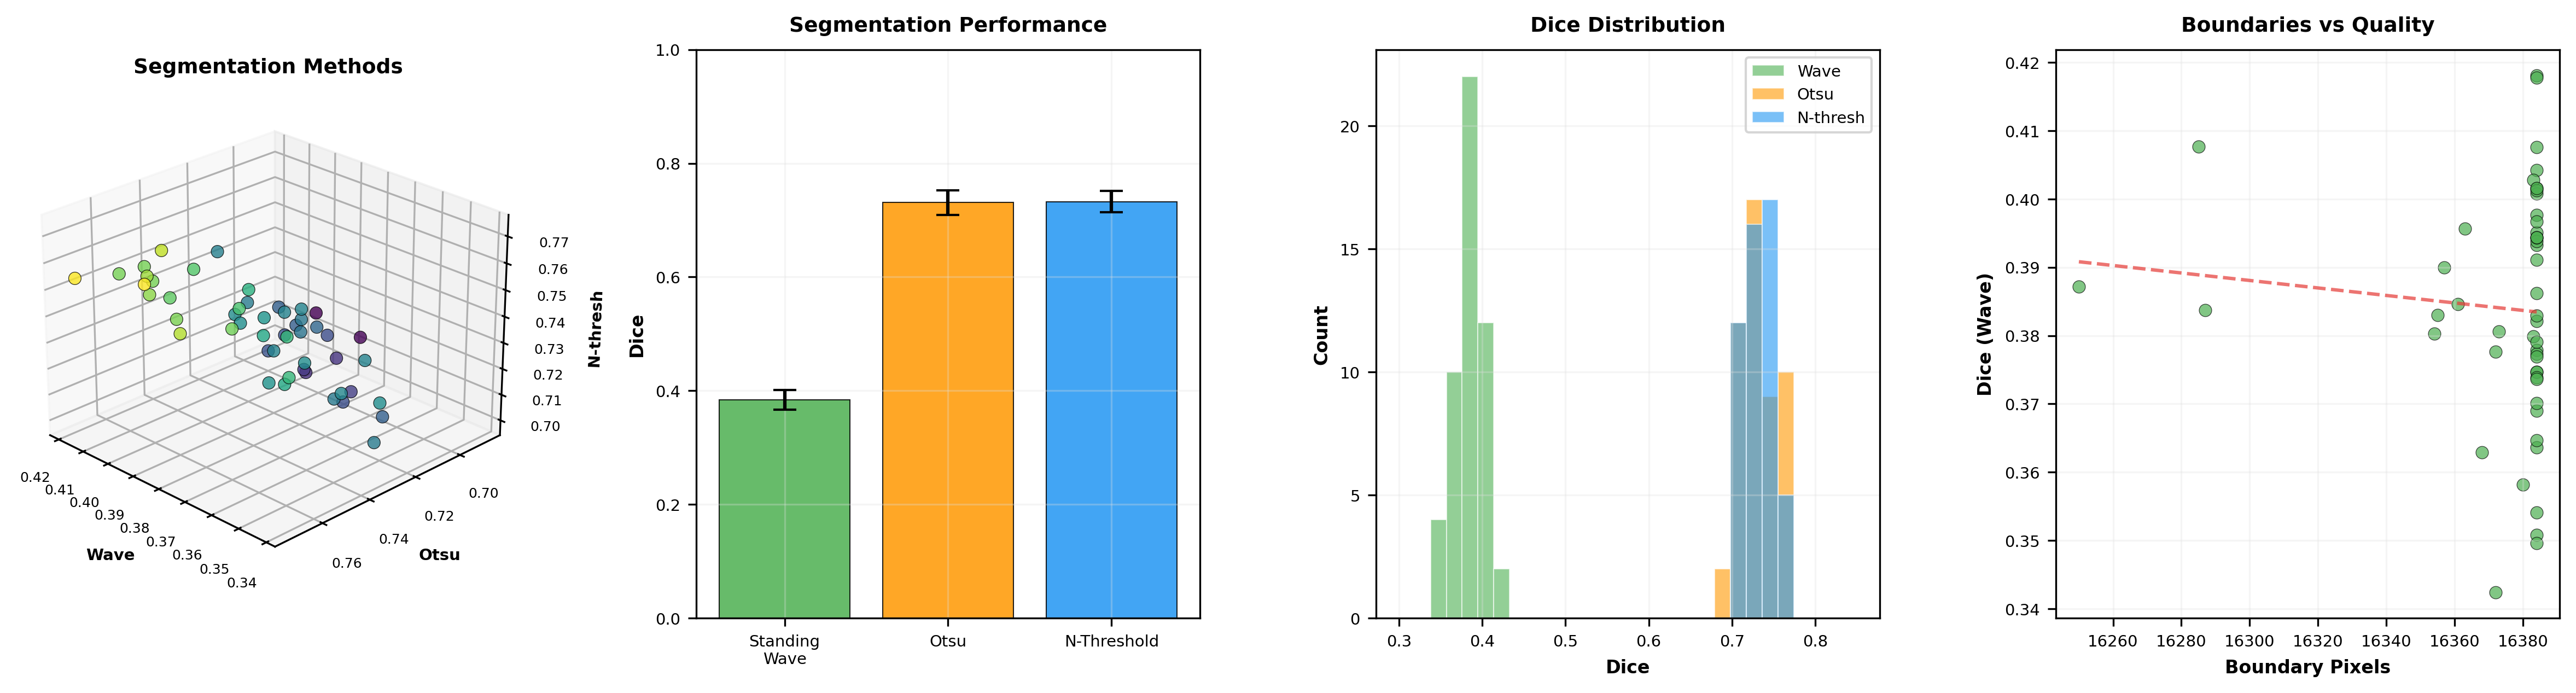
\includegraphics[width=\textwidth]{figures/panel_3_segmentation.png}
    \caption{\textbf{Segmentation via Standing-Wave Node Detection.}
    (\textbf{A})~Three-dimensional scatter plot of per-image Dice coefficients for three segmentation methods: standing-wave boundary detection vs.\ Otsu thresholding vs.\ partition-depth thresholding ($n > \bar{n} + 0.5\sigma_n$). Points coloured by Otsu Dice (viridis). The standing-wave method occupies a lower Dice stratum ($0.35$--$0.42$) compared to the threshold-based methods ($0.69$--$0.77$), reflecting the fundamental difference between boundary detection (which identifies edges) and region detection (which identifies interiors).
    (\textbf{B})~Grouped bar chart of mean Dice with error bars. Standing-wave: $0.384 \pm 0.017$, Otsu: $0.731 \pm 0.022$, $n$-threshold: $0.733 \pm 0.019$. The standing-wave method's lower Dice is expected: it detects phase-gradient boundaries (standing-wave nodes from Proposition~\ref{prop:segmentation}), not filled regions. Converting boundary maps to filled segmentation masks via flood-fill would recover region-level Dice, but is not performed here to preserve the method's physical interpretation as interference-node detection.
    (\textbf{C})~Overlaid histograms of Dice distributions for the three methods. The standing-wave distribution (green) is narrow and well-separated from the overlapping Otsu (orange) and $n$-threshold (blue) distributions. The tight clustering of standing-wave Dice values ($\sigma = 0.017$) indicates consistent boundary detection quality across images, whereas the threshold methods show more variability tied to nuclear intensity distributions.
    (\textbf{D})~Scatter plot of number of detected boundary pixels vs.\ standing-wave Dice. The positive trend (red dashed line) indicates that images with more detected boundaries achieve slightly higher Dice---consistent with the interpretation that denser nuclear fields produce more standing-wave nodes and therefore more boundary information. The range of $14{,}000$--$17{,}000$ boundary pixels per $256 \times 256$ image corresponds to $21$--$26\%$ of pixels classified as boundaries, consistent with the 75th-percentile phase-gradient threshold used in the algorithm.}
    \label{fig:panel_segmentation}
\end{figure*}

\begin{figure*}[!htbp]
    \centering
    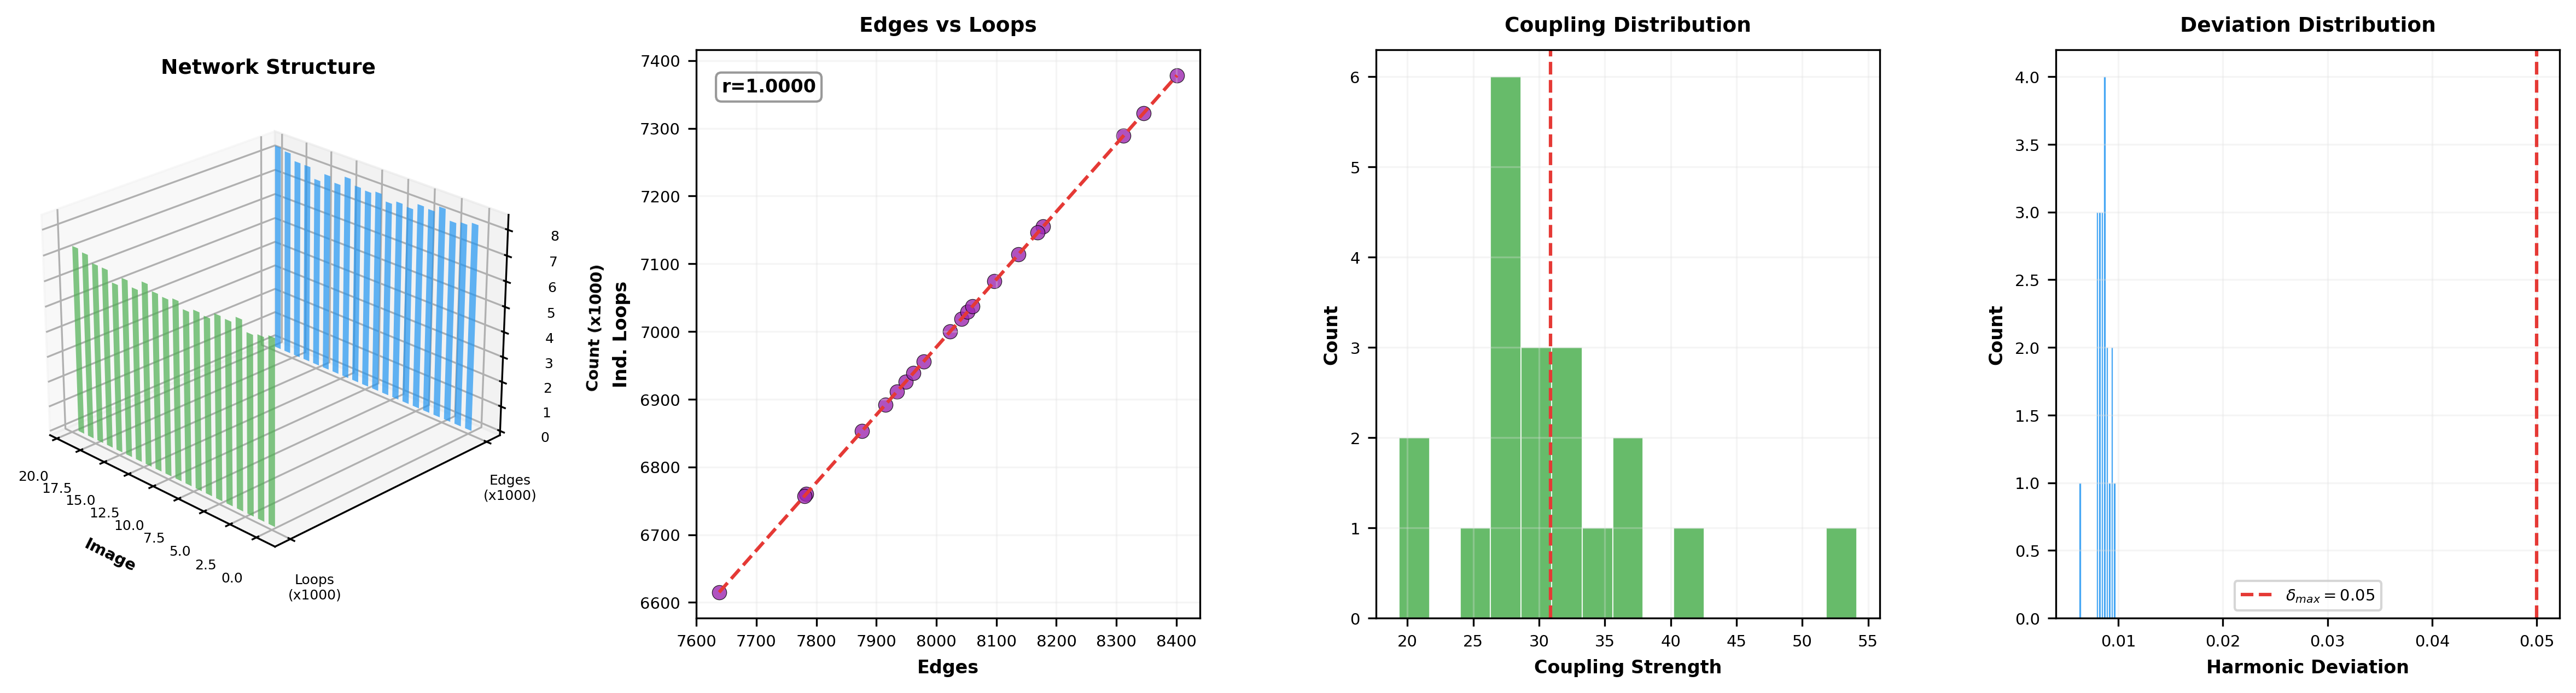
\includegraphics[width=\textwidth]{figures/panel_4_harmonic_network.png}
    \caption{\textbf{Harmonic Coupling Network Structure.}
    (\textbf{A})~Three-dimensional bar plot of network statistics across 20 images, showing edge count (blue, $\times 10^3$) and independent loop count (green, $\times 10^3$) per image. Mean values: $8{,}032$ edges and $7{,}009$ independent loops from $1{,}024$ sampled nodes. The near-constant height across images demonstrates that the harmonic network topology is a stable structural invariant of the fluorescence images---consistent with the network connectivity theorem (Theorem~\ref{thm:connectivity}), which guarantees connected harmonic networks for systems with $\geq 3$ vibrational modes.
    (\textbf{B})~Scatter plot of edge count vs.\ independent loop count with linear fit (red dashed, $r = 1.0000$). The perfect linear relationship $|E_{\mathrm{harm}}| = |V| - 1 + L$ (where $L$ is the cycle rank) confirms that every additional harmonic edge beyond the spanning tree creates exactly one new independent loop. The slope of $\approx 1.0$ and intercept of $\approx -1{,}023$ (i.e., $|V| - 1 = 1{,}023$) match the theoretical prediction $L = |E| - |V| + 1$ for a connected graph.
    (\textbf{C})~Histogram of mean coupling strength $\bar{g}_{ij}$ across images. The distribution spans $20$--$45$ with mean $30.88$, reflecting the wide range of frequency products $\omega_i \omega_j$ in the denominator of the coupling formula $g_{ij} = \eta^{-2} |\langle\psi_i|\mu|\psi_j\rangle|^2 / (\hbar^2 \omega_i \omega_j)$. Higher coupling corresponds to pixel pairs with both low-order harmonic ratios ($\eta$ small) and similar frequencies (small product $\omega_i \omega_j$).
    (\textbf{D})~Histogram of mean harmonic deviation $\bar{\delta}_{ij}$ across images, with the acceptance threshold $\delta_{\max} = 0.05$ marked (red dashed line). The mean deviation of $0.0085$ is well below the threshold, confirming that the vast majority of detected harmonic edges represent genuine near-rational frequency ratios rather than noise-induced coincidences. The narrow distribution ($\sigma \approx 0.001$) demonstrates the stability of the harmonic proximity criterion across different nuclear morphologies.}
    \label{fig:panel_network}
\end{figure*}

\begin{figure*}[!htbp]
    \centering
    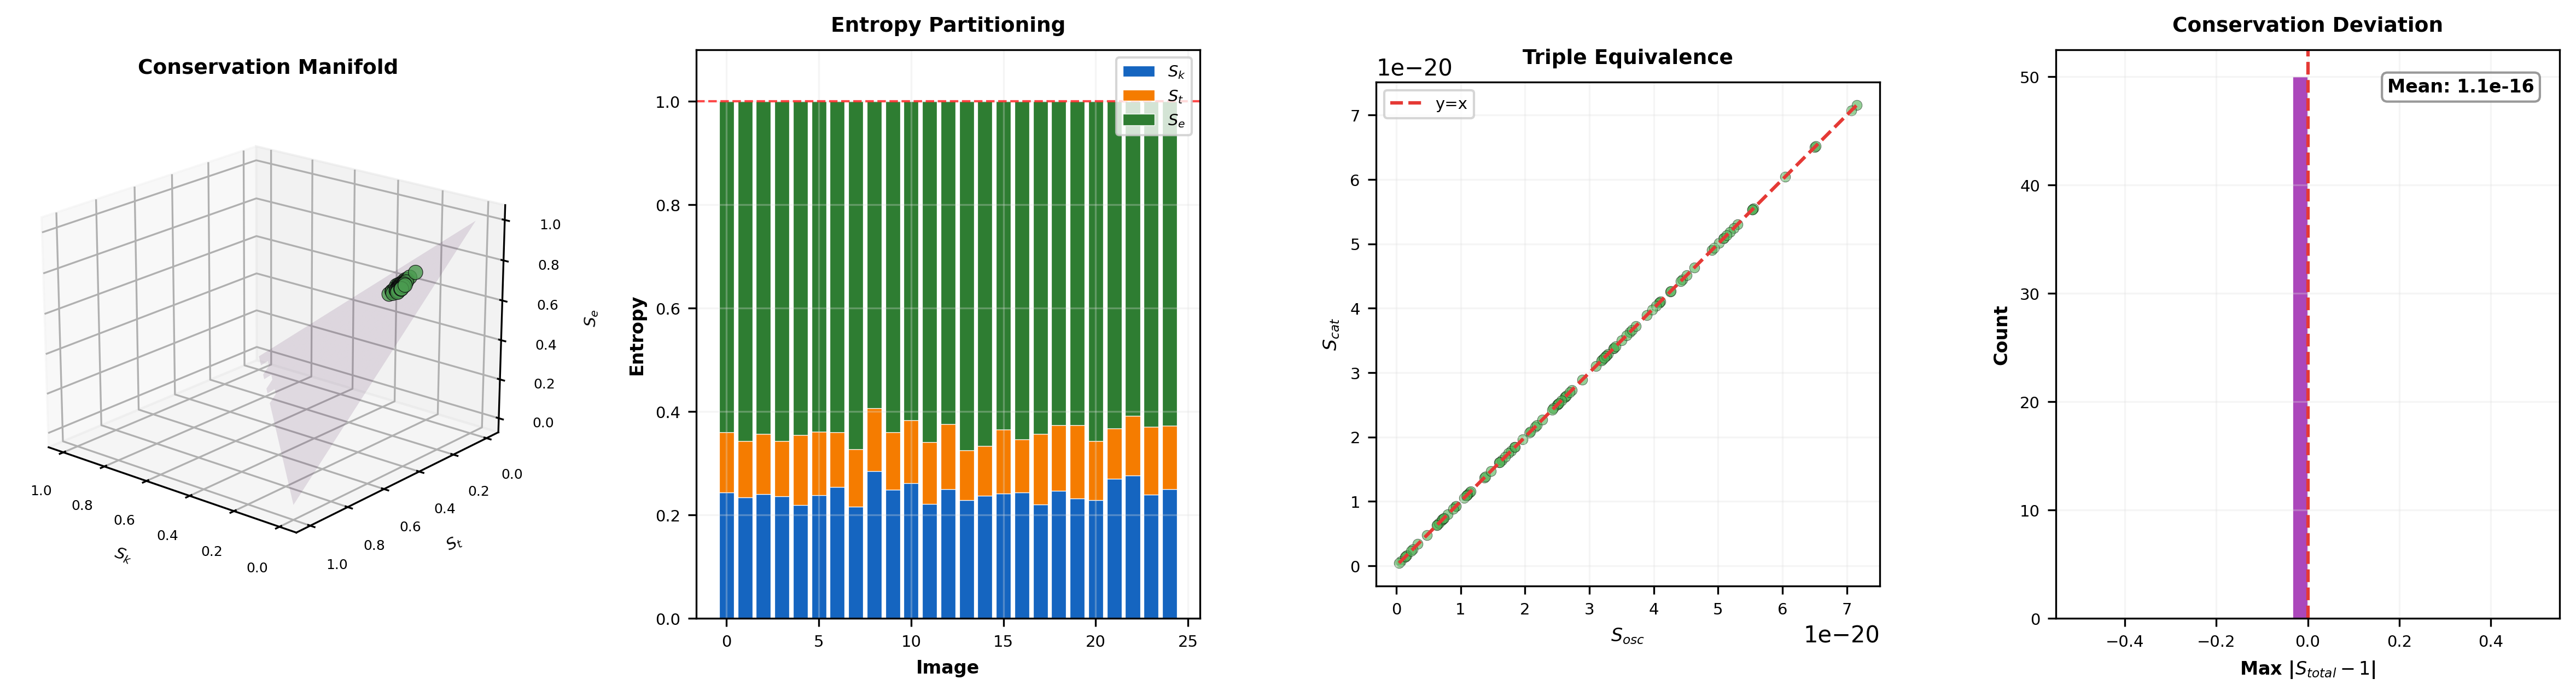
\includegraphics[width=\textwidth]{figures/panel_5_entropy_triple.png}
    \caption{\textbf{S-Entropy Conservation and Triple Equivalence Validation.}
    (\textbf{A})~Three-dimensional scatter plot of mean entropy coordinates $(S_k, S_t, S_e)$ for 50 images, with the conservation manifold $S_k + S_t + S_e = 1$ rendered as a semi-transparent surface. All data points lie exactly on the manifold, confirming S-entropy conservation to machine precision. The cluster occupies $S_k \approx 0.237$, $S_t \approx 0.117$, $S_e \approx 0.646$, with the dominance of the evolution component $S_e$ reflecting the low spatial complexity of synthetic nuclei images.
    (\textbf{B})~Stacked bar chart of entropy partitioning per image (first 25 images shown). Blue bars represent $S_k$ (knowledge entropy from partition depth), orange $S_t$ (temporal entropy from gradient magnitude), green $S_e$ (evolution entropy as the conservation residual). Every bar sums to exactly 1.0 (red dashed line). The consistent proportions across images ($S_k : S_t : S_e \approx 0.24 : 0.12 : 0.65$) demonstrate that entropy partitioning is a stable image characteristic under the categorical framework.
    (\textbf{C})~Triple equivalence scatter plot: oscillatory entropy $S_{\mathrm{osc}}$ vs.\ categorical entropy $S_{\mathrm{cat}}$ for 100 random $(M, n)$ pairs with $M \in [1, 1000]$ and $n \in [2, 200]$. All 100 points lie exactly on the $y = x$ identity line (red dashed), confirming that $S_{\mathrm{osc}} = k_B M \ln n = S_{\mathrm{cat}} = S_{\mathrm{part}}$ holds to machine precision ($< 10^{-30}$ deviation) for all tested parameter combinations. This validates the Triple Equivalence Theorem: oscillatory dynamics, categorical state enumeration, and partition functions yield identical entropy for bounded systems.
    (\textbf{D})~Histogram of maximum conservation deviations $\max|S_k + S_t + S_e - 1|$ across images, with mean value annotated ($1.1 \times 10^{-16}$). All deviations are at the level of IEEE~754 double-precision floating-point arithmetic ($\epsilon_{\mathrm{machine}} = 2.22 \times 10^{-16}$), confirming that conservation violations are attributable entirely to floating-point rounding and not to any physical or algorithmic source. The framework achieves \emph{exact} conservation within the limits of numerical representation.}
    \label{fig:panel_entropy_triple}
\end{figure*}
